\Section{natlog-mono}{Monotonicity Calculus}

%
% Intro with Algebra
%
We begin this section by reviewing monotonicity in its familiar context:
  monotonicity of algebraic functions.
For example, $f(x) = e^x - 1$ is a \textit{monotone} function -- as we increase $x$,
  the value of $f(x)$ monotonically increases.
A function may also be \textit{antitone}: $f(x) = e^{-x}$ is antitone, since 
  the value of $f(x)$ decreases monotonically as $x$ increases.
Lastly, a function can be \textit{nonmonotone} -- distinct from antitone -- if
  it is neither monotone nor antitone.

Visually, the plots below show a monotone function ($e^x - 1$) and an antitone 
  function ($e^{-x}$).
We will appeal to analogous visualizations when we move towards working with
  language.

\begin{center}
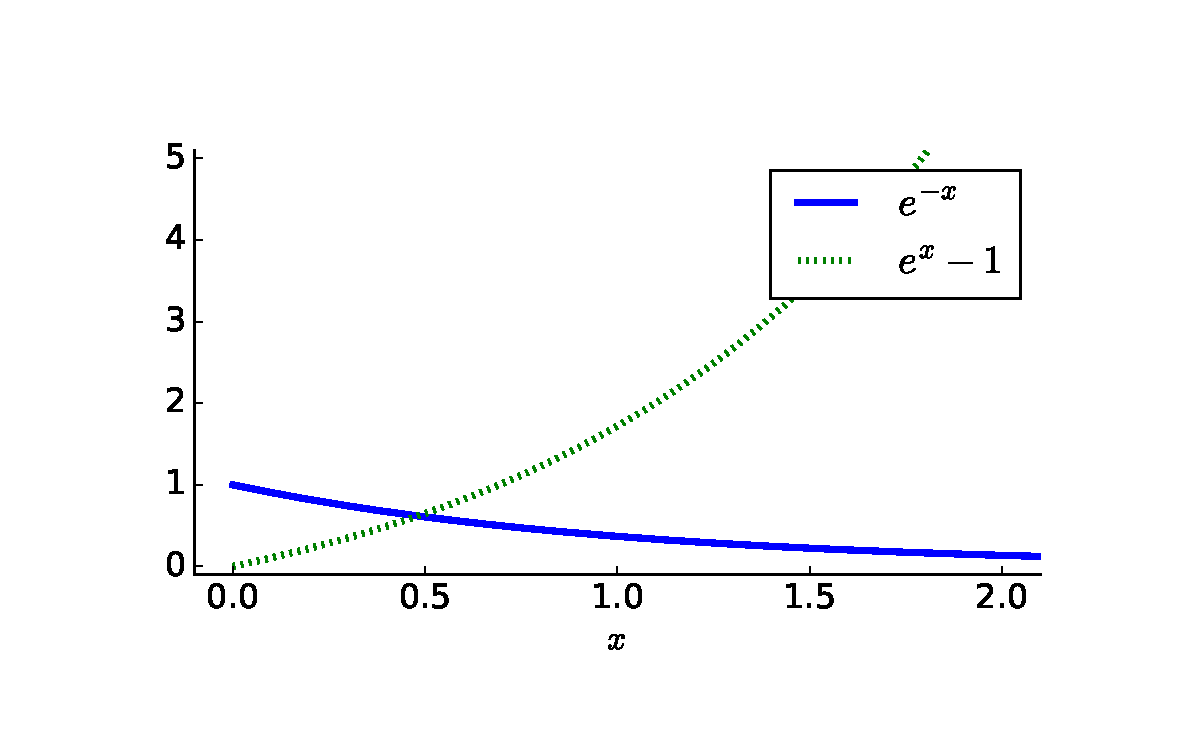
\includegraphics[height=7cm]{img/monotonicity_math.pdf}
\end{center}


% Sales Pitch
Monotonicity is an appealing tool because it lets us reason about functions
  without having to evaluate them.
To illustrate, we can define an arbitrarily complex function $f : \R \rightarrow \R$,
  which we are told is monotone.
Without evaluating the function, we are able to conclude that
  $f(x + 1) > f(x)$.
This is precisely the type of tool we would like to use to manipulate language:
  constructing a concrete interpretation of language -- like evaluating 
  a complex function -- is at best undesirable and at worst impossible.
However, if we know some properties about the ``monotonicity'' of the language,
  we can manipulate the text such that we preserve some key relations
  between the original and our mutated text -- analogous to the greater-than
  relation in our algebraic example.

This analogy is much more direct than it may at first appear:
  we defined a class of functions in 
  \refsecs{natlog-denotations-other}{natlog-denotations-quantifiers},
  and monotonicity calculus will be the calculus of valid inferences that
  we can draw from reasoning about the monotonicity of these functions.
%  monotonicity calculus reasons about the functions defined in 
The remainder of this section will explore how to apply monotonicity to
  the denotational semantics in \refsec{natlog-denotations},
  and then introduce reasoning about exclusion (\refsec{natlog-mono-exclusion}).
The section will conclude by introducing the notion of \textit{polarity},
  and exploring how to compose monotone functions in a sentence.



%
% Monotonicity in Language
%
\Subsection{natlog-mono-general}{Monotonicity in Language}

In generality, a monotone function is a function between partially-ordered sets
  that preserves the given order.
For a function $f$ with domain $\bX$ and range $\bY$, we define a partial order over
  $\leq_X$ and $\leq_Y$.
This function is monotone iff:

\begin{equation}
  \forall x_1, x_2 \in \bX ~~ \textrm{such that} ~~ x_1 \leq_X x_2; ~~  f(x_1) \leq_Y f(x_2)
\end{equation}

We note from \refsec{natlog-denotations} that, by and large, sentences 
  are constructed by composing one or more functions (e.g., verbs, operators).
To reason about whether these functions are monotone (or, by extenstion, antitone),
  we need to show that each of our domains forms a partial order we can define
  monotonicity against.

First: the domain of noun denotations: $\sD_e$ (or, $e$).
We define our partial order $\leq_e$ to be the subset operator: $\subseteq$.
That is, if the denotation of a word is completely contained in the denotation of
  another word, we consider the first word to be ``less than'' the second.
This is intuitively encoding hypernymy as a partial order.
For example, $\llbracket cat \rrbracket$ $\leq_e$ $\llbracket feline \rrbracket$ because
  any entity which is a cat is also necessarily a feline.

Second: the domain of truth values: $\sD_t$ (or, $t$).
Here, we axiomatically define a partial order $\leq_t$ to be:\footnote{
    The elegance of the interpretation of false as the empty set and true as a singleton
    set becomes clear here: we can define the partial order over truth values to be the same
    subset operator as the partial order over noun denotations.
    }

\begin{align*}
  false &\leq_t false \\
  false &\leq_t true \\
  true &\leq_t true \\
\end{align*}

The very important observation to make at this point is that
  \textbf{the partial order $\leq_t$ corresponds exactly to the material conditional $\supset$}.
So, for any two propositions $A$ and $B$, $A$ entails $B$ ($A \supset B$) is the same
  as $A \leq_t B$.
This is the key insight tying together the concepts of monotonicity and entailment.
We also point out the unfortunate fact that the symbol for the material conditional
  is the same as the superset symbol, which would seem to evoke ``greater than'' rather
  than the ``less than'' it actually corresponds to.
Unfortunately, this dissertation is not the place to redefine either of these symbols.

Lastly: we must define a partial order over our inductively defined function types.
A function is less than another function if, for all
  values in the domain of the functions, the value of the first function is less than
  the value of the second.
Formally: for two functions $f$ and $g$ with the same domain and range $\bX \rightarrow \bY$,
  we say $f \leq_f g$ iff:

\begin{equation}
  \forall x \in \bX; ~~ f(x) \leq_Y g(x)
\end{equation}

For the remainder of this thesis, we will collapse all of these partial orders
  -- $\leq_e$, $\leq_t$, and $\leq_f$ -- into
  a single symbol: \forward.



% Monotonicity is entailment-preserving
\paragraph{Monotonicity is Entailment-Preserving}
The most important insight from the partial orders above is that our partial order
  over truth values corresponds exactly to entailment.
Although ``entailment'' is not particularly well-defined for the other denotation
  types (i.e., does \ww{cat} entail \ww{animal}?), for the purposes of monotonicity
  calculus and natural logic we will take the symbol \forward\ to be entailment.\footnote{
    This is, again, not to be confused with the symbol for entailment in propositional
    logic: $\supset$.
  }
By extension, we can define $A \reverse B$ to mean that $B \forward A$, and define
  \equivalent\ to be equivalence.
That is to say, $A \equivalent B$ is the same as $A \forward B$ and $B \forward A$.

This means that monotone functions are entailment preserving.
If a sentence is true, and the function used to construct its denotation (i.e., truth)
  is monotone with respect to the denotation of a word, then replacing that word with
  another word whose denotation is a superset of the original word will maintain
  the truth of the sentence.
Taking a concrete example: \ww{all} (a function $e \rightarrow (e \rightarrow t)$)
  is antitone in its first argument and monotone in its second.
So, the sentence \ww{all cats drink milk} is antitone with respect to \ww{cats} and
  monotone with respect to \ww{drink milk}.
Furthermore, we know that 
  $\llbracket drink ~ milk\rrbracket \forward \llbracket drink~dairy\rrbracket$
  because $\llbracket milk\rrbracket \forward \llbracket dairy\rrbracket$.
Therefore, by the definition of monotonicity, we can replace \ww{drink milk} with
  \ww{drink dairy} and the resulting sentence (\ww{all cats drink dairy})
  is guaranteed to be true if the original sentence was true.

The fact that quantifiers and other operators in natural language have this
  property of monotonicity is wonderfully convenient.
Grounding an interpretation for \ww{all cats drink milk} would be rather
  difficult in the general case -- and certainly difficult for longer utterances.
But by appealing to the monotonicity of quantifiers, we do not need to ground
  the sentence to run an entailment proof on it.
Antitone functions behave analogously to monotone functions, but with the 
  direction of the lexical mutation reversed.
For example, if \ww{all cats drink milk}, we can infer that 
  \ww{all kittens drink milk} because 
  $\llbracket cat \rrbracket \reverse \llbracket kitten\rrbracket$.

Like the visualization with monotone algebraic functions earlier in the section,
  we can visualize monotonicity over denotations.
In the chart below, the $x$ axis is an ordering over denotations.\footnote{
    In general this is a partial order; however, partial orders are difficult
    to plot on an axis.
    }
The $y$ axis is the ordering over truth values.
We are plotting two functions: \ww{all $x$ drink milk} -- antitone in $x$; and
  \ww{some $x$ bark} -- monotone in $x$:

\begin{center}
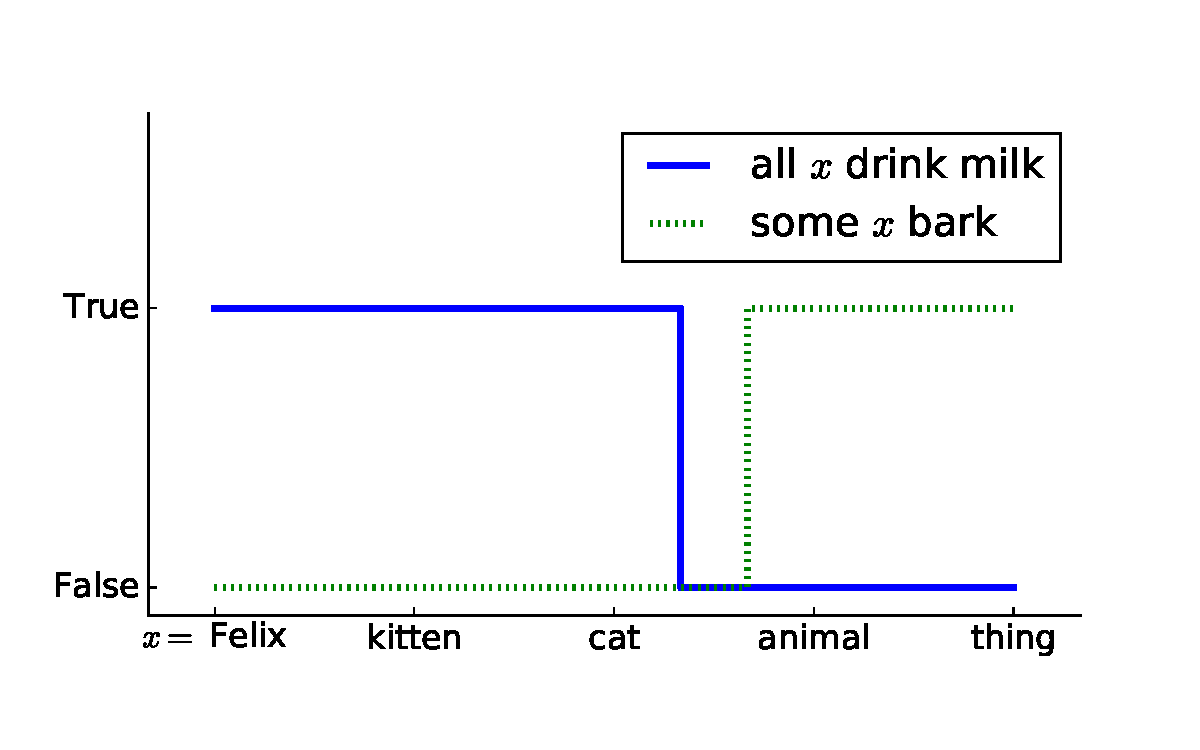
\includegraphics[height=7cm]{img/monotonicity_lex_all.pdf}
\end{center}

% Back to proof theory for a bit
\paragraph{Monotonicity Calculus as a proof theory}
At this point, we can begin looking at monotonicity calculus as the sort of natural
  logic proof system we demonstrated at the beginning of the chapter.
For example, our inference from \ww{the cat ate a mouse} to 
  \ww{the carnivore ate an animal} could be formally justified with the following proof.
We note that the quantifier \ww{the} -- like \ww{some} -- is monotone in both
  of its arguments.

\[
\begin{nd}
\hypo {1} {\ww{The cat ate a mouse.}}
\have {2} {\ww{The cat ate a rodent.}}         \by{\denote{mouse} \forward\ \denote{rodent}}{1}
\have {3} {\ww{The cat ate an animal.}}        \by{\denote{rodent} \forward\ \denote{animal}}{2}
\have {4} {\ww{The feline ate an animal.}}     \by{\denote{cat} \forward\ \denote{feline}}{3}
\have {5} {\ww{The carnivore ate an animal.}}  \by{\denote{carnivore} \forward\ \denote{animal}}{4}
\end{nd}
\]

However, we still lack the tools to infer that \ww{no carnivore ate an animal} is false
  given our premise.
For this, we need a theory of how to reason with \textit{exclusion} -- which we will
  review in the next section.
Furthermore, our theory currently does not handle nested quantification.
In \refsec{natlog-mono-polarity}
  we introduce \textit{Polarity} and the mechanism for propagating monotonicity information
  to determine the ``monotonicity'' of a sentence composed of multiple quantifiers.



%
% Exclusion
%
\Subsection{natlog-mono-exclusion}{Exclusion}
Although the monotonicity calculus of \newcite{key:1991valencia-natlog} can already
  do a range of interesting inferences, it is nonetheless still a very restricted
  logic.
This section reviews work by \newcite{key:2008maccartney-natlog} and
  \newcite{key:2014icard-natlog} on how natural logic can be extended to handle
  negation and antonomy by reasoning about \textit{exclusion}.
Much of the notation is adapted from \newcite{key:2014icard-natlog}.


\begin{figure}[th]
\begin{center}
\begin{tabular}{ccc}
  \forwardVenn & \reverseVenn     & \equivalentVenn \\
  \negateVenn  & \alternateVenn   & \coverVenn \\
               & \independentVenn &

\end{tabular}
\end{center}
\longcaption{An enumeration of the possible relations between two sets of denotations}{
\label{fig:natlog-setrelations}
An enumeration of the possible relations between two sets $\varphi$ (dark green) and
$\psi$ (light yellow).
The top three relations are the simple relations used in monotonicity calculus; the middle three
  are relevant for exclusion; the bottom relation denotes the case where nothing of interest
  can be said about the two sets.
}
\end{figure}


% Partially distributive lattice
The foundations for exclusion come from the observation that there are more relations
  you can define between sets than the subset / superset / equality relations
  used in the monotonicity calculus described in \refsec{natlog-mono-general}.
Given a set $\varphi$ and a set $\psi$, these relations are enumerated in \reffig{natlog-setrelations}.
The top row correspond to the relations we are familiar with (\forward, \reverse, \equivalent)
  along with their interpretation in natural logic.
The middle row describes the three relations relevant for exclusion.
The bottom row describes the independence relation, meaning that nothing of interest
  can be said about the two relations.

We review each of these four new relations, and their interpretation for our three
  entity types: denotations, truth values, and functions.

First, however; to extend these definition beyond sets, and therefore beyond denotations
  to truth values and to functions, we introduce a bit of notation.
In particular, we define a \textit{partially distributive lattice}.
This is  a 5-tuple:
  $(\bD, \lor, \land, \bot, \top)$,
  consisting of a domain $\bD$ (the set of entities in the lattice), two binary operators
  $\lor$ and $\land$ corresponding to a generalized sense of \textit{maximum} and
  \textit{minimum} respectively,\footnote{
    $\lor$ and $\land$ must also be commutative, associative, and idempotent; and they must
    distribute over each other.
  } and two elements in $\bD$, $\bot$ and $\top$, corresponding
  intuitively to the smallest and largest element of $\bD$, respectively.

For denotations, we define this lattice as follows, mirroring previous sections.
\begin{lquote}
$\bD$ is the power set of all denotations in $\sD_e$. \\
$\lor$ is the union operator: $\cup$. \\
$\land$ is the intersect operator: $\cap$. \\
$\bot$ is the empty set: $\{\}$. \\
$\top$ is the full domain of denotations: $\sD_e$.
\end{lquote}

For truth values, we define the lattice straightforwardly as:
\begin{lquote}
$\bD$ is the set $\{0, 1\}$, where 0 corresponds to false and 1 corresponds to true. \\
$\lor$ maximum (i.e., $1 \lor 0 = 1$) \\
$\land$ minimum (i.e., $1 \land 0 = 0$) \\
$\bot$ is false: $0$. \\
$\top$ is true: $1$.
\end{lquote}


Defining this lattice over functions is a bit more verbose, but intuitively analogous
  to the denotation and truth value cases.
Since the range of our functions is ordered (e.g., the domain of truth values $t$ is ordered
  in a function $e \rightarrow t$),
  and the range has a maximum and minimum element (e.g., true and false respectively for $t$),
  we can from this define our ``largest'' and ``smallest'' functions $\top$ and $\bot$.
$\top$ is the function which takes any element in its domain, and maps it to
  the maximum element in the function's range.
As a concrete example, for a function $e \rightarrow t$ this corresponds to a tautology --
  e.g., \ww{$x$ is $x$} maps everything to $\top$ in the domain of truth values
  (i.e., \textit{true}).
The function corresponding to $\bot$, conversely, maps every element in its domain 
  to the smallest element (i.e., $\bot$) in the function's range.

We further define the $\lor$ and $\land$ of two function to be the element-wise $\lor$
  and $\land$ of the functions.
That is, for functions $f:A \rightarrow B$ and $g:A \rightarrow B$, 
  $h = f \lor g$ iff $\forall x, h(x) = f(x) \lor g(x)$.
$f \lor g$ is defined analogously.
To summarize, the lattice for a function $f:A \rightarrow B$ is:

\begin{lquote}
$\bD$ is the set of all functions from $A$ to $B$. \\
$\lor$ is the element-wise $\lor$ of the functions. \\
$\land$ is the element-wise $\land$ of the functions. \\
$\bot$ is the function mapping any $A$ to $\bot$ in $B$. \\
$\bot$ is the function mapping any $A$ to $\top$ in $B$. \\
\end{lquote}

We can use our definition of this lattice to formally define the new relations in
  \reffig{natlog-setrelations}, and give new interpretations to the relations
  from above.


% Negation
\paragraph{Negation (\negate)}
From \reffig{natlog-setrelations}, two sets are in \textit{negation} 
  if the union of the sets is the entire domain, and the
  intersection of the sets is empty.
That is, for two sets $\varphi$ and $\phi$,
  $\varphi \cup \psi = \sD$ and $\varphi \cap \psi = \{\}$.
Generalizing this to our lattice definition above, we say that two terms
  are in negation with each other iff
  $x \lor y = \top$ and $x \land y = \bot$.
As the name would imply, the most natural examples of negation appearing for 
  pairs of denotations usually involve some sort of morphological negation:
\begin{lquote}
\denote{cat} \negate\ \denote{noncat} \\
\denote{living thing} \negate\ \denote{nonliving thing} \\
\denote{possible thing} \negate\ \denote{impossible thing} \\
\end{lquote}


For truth values, negation (unsurprisingly) corresponds to logical negation.
We can recover the truth table for negation straightforwardly from the definition
  of the lattice, recalling that $\lor$ is $\max$, $\land$ is $\min$, $\top$ is 1,
  and $\bot$ is 0: 
  
\begin{center}
\begin{tabular}{cc|cc:c}
  $x$ & $y$ & $x \lor y$ & $x \land y$    & $x \lor y = \top~$ and $~x \land y = \bot$ \\
  \hline
  0   &  0  &    0       &      0         &              0                \\
  0   &  1  &    1       &      0         &              1                \\
  1   &  0  &    1       &      0         &              1                \\
  1   &  1  &    1       &      1         &              0                \\
\end{tabular}
\end{center}

The definition of negation for functions likewise follows.
Two functions $f$ and $g$ are then negations of each other ($f$ \negate\ $g$)
  iff elementwise $\max(f, g)$ (i.e., $f \lor y$) always maps to $\top$, 
  and $\min(f, g)$ (i.e., $f \land y$) always maps to $\bot$.
To illustrate with a concrete example, the functions \ww{$x$ is living} and
  \ww{$x$ is nonliving} are in negation, since for any $x$ it is either true that
  it is living, or it's true that it is nonliving; and, for any $x$, it is
  it is never true that it is both living and nonliving.
This extends trivially to quantifiers.
For example, \ww{no} and \ww{some} are negations of each other.


The next two relations -- alternation (\alternate) and cover (\cover) -- can be
  though of as holding one, but not both of the conditions of negation.
In particular, two entities in the negation relation are also necessarily in the
  alternation and cover relations.


% Alternation
\paragraph{Alternation (\alternate)}
Alternation can be thought of as another form of negation, which is weaker in
  some important respects which will become clear later.
In the generalized case, two entities are in alternation iff $x \land y = \bot$.

Two denotations are in \textit{alternation} if their intersection is empty.
That is, for sets $\varphi$ and $\psi$, $\varphi \cap \psi = \{\}$,
  but unlike negation we do not know anything about their union.
This is commonly the relation which holds between antonyms and otherwise
  contradictory nouns:

\begin{lquote}
\denote{cat} \alternate\ \denote{dog} \\
\denote{genius} \alternate\ \denote{idiot} \\
\denote{good deed} \alternate\ \denote{bad deed} \\
\end{lquote}


For truth values, alternation equates pragmatically to negation in the context of
  proving entailment.
That is, false \alternate\ false is true (whereas false \negate\ false is false);
  however, this is only relevant if we are assuming that our premise is false.
Since we are (axiomatically) assuming that our premise is true, this case will never
  arise, and the truth table looks otherwise equivalent to full negation:
 

\begin{center}
\begin{tabular}{cc|cc:c}
  $x$ & $y$ & $x \lor y$ & $x \land y$    & $x \land y = \bot~$ \\
  \hline
  0   &  0  &    0       &      0         &              1                \\
  0   &  1  &    1       &      0         &              1                \\
  1   &  0  &    1       &      0         &              1                \\
  1   &  1  &    1       &      1         &              0                \\
\end{tabular}
\end{center}


The intuition for when functions are in alternation becomes potentially hairy, but
  not awful.
Adjective antonyms are a clear example: \ww{hot $x$} \alternate\ \ww{cold $x$}, since
  for any $x$ we know that $x$ is not both hot and cold.
The quantifiers \ww{all} and \ww{no} are similarly in alternation.



% Cover
\paragraph{Cover (\cover)}
In many ways, cover is the most strange of the relations in this section.
For \textit{nearly} all intents and purposes, this relation indicates 
  neither entailment nor negation between its two entities, but it occasionally
  conveys a hint of negation.
Concretely, cover behaves as negation
  when reasoning about a counter-factual premise -- e.g.,
  if in an entailment chain you have negated your premise -- and are now continuing
  to reason about this presumed false intermediate statement.
Formally, two entities are in the cover relation iff $x \lor y = \top$.

For denotations, this is a quintessentially rare case ($\varphi \cup \psi = \sD$), 
  and examples which don't amount to outright negation are almost always a bit contrived:
\begin{lquote}
\denote{animal} \cover\ \denote{non-cat} \\
\denote{smartphone} \cover\ \denote{non-iphone} \\
\end{lquote}


The behavior of the cover relation becomes a bit more apparent in the case of
  truth values.
Analogous to how alternation (\alternate) was pragmatically negation when the premise
  is true, cover is pragmatically negation when the premise is \textit{false}.
We will, of course, never assume that the premise in a proof is false; but certainly
  intermediate steps in the proof may find us with a presumed false statement.
In these cases, the cover relation allows us to ``negate'' this false statement.

\begin{center}
\begin{tabular}{cc|cc:c}
  $x$ & $y$ & $x \lor y$ & $x \land y$    & $x \lor y = \top~$ \\
  \hline
  0   &  0  &    0       &      0         &              0                \\
  0   &  1  &    1       &      0         &              1                \\
  1   &  0  &    1       &      0         &              1                \\
  1   &  1  &    1       &      1         &              1                \\
\end{tabular}
\end{center}

The cover relation is virtually unseen for functions, although of course the definition
  still carries over fine.



% Independence
\paragraph{Independence (\independent)}
The last relation is independence, which corresponds to no relation holding purely
  by virtue of the constructed lattice.
This is the case for, e.g.,
\begin{lquote}
\denote{cat} \independent\ \denote{black animal} \\
\denote{happy} \independent\ \denote{excited} \\
\denote{play} \independent\ \denote{run} \\
\end{lquote}



% Old relations
\paragraph{The old relations (\forward, \reverse, \equivalent)}
The relations from the simple monotonicity calculus in \refsec{natlog-mono-general}
  of course also have generalized interpretations in the context of our lattice.
The behavior remains identical to before.
The generalized definitions are:
\begin{lquote}
$x \forward y$ iff $x \land y = x$ \\
$x \reverse y$ iff $x \lor y = x$ \\
$x \equivalent y$ iff $x \land y = x~$ and $~x \lor y = x$ \\
\end{lquote}




%
% Composition
%
\Subsection{natlog-mono-composition}{Proofs with Exclusion}


\begin{table}[t]
	\begin{center}
	\begin{tabular}{|c||c|c|c|c|c|c|c|}
    \hline
    $\bowtie$ & $\equivalent$ & $\forward$ & $\reverse$ & $\negate$ & $\alternate$ & $\cover$ & $\independent$ \\
    \hline
    $\equivalent$ & $\equivalent$ & $\forward$ & $\reverse$ & $\negate$ & $\alternate$ & $\cover$ & $\independent$ \\
    $\forward$ & $\forward$ & $\forward$ & $\independent$ & $\alternate$ & $\alternate$ & $\independent$ & $\independent$ \\
    $\reverse$ & $\reverse$ & $\independent$ & $\reverse$ & $\cover$ & $\independent$ & $\cover$ & $\independent$  \\
    $\negate$ & $\negate$ & $\cover$ & $\alternate$ & $\equivalent$ & $\reverse$ & $\forward$ & $\independent$  \\
    $\alternate$ & $\alternate$ & $\independent$ & $\alternate$ & $\forward$ & $\independent$ & $\forward$ & $\independent$  \\
    $\cover$ & $\cover$ & $\cover$ & $\independent$ & $\reverse$ & $\reverse$ & $\independent$ & $\independent$  \\
    $\independent$ & $\independent$ & $\independent$ & $\independent$ & $\independent$ & $\independent$ & $\independent$ & $\independent$ \\
    \hline
	\end{tabular}
	%(caption)
	\caption{The join table as taken from \newcite{key:2012icard-natlog}.}
  {
    The join table as taken from \newcite{key:2012icard-natlog}.
    Entries in the table are the result of joining a row with a
      column.
    Note that the $\independent$ always joins to yield $\independent$,
    and $\equivalent$ always joins to yield the input relation.
		\label{tab:natlog-jointable}
	}
	\end{center}
\end{table}



We showed how to run simple proofs in monotonicity calculus in 
  \refsec{natlog-mono-general} by simply appealing to the transitivity of the
  $\forward$ relation.
In effect, we implicitly defined a transitivity table, or \textit{join table},
  for how to assess the relation between $x$ and $z$ if we know the relation
  between $x$ and $y$, and between $y$ and $z$.
We then \textit{join} these two relations together with the $\bowtie$ operator defined
  below to obtain the final relation between $x$ and $z$:
	
\begin{center}
\begin{tabular}{|c||c|c|c|}
  \hline
  $\bowtie$ & $\equivalent$ & $\forward$ & $\reverse$ \\
  \hline
  $\equivalent$ & $\equivalent$ & $\forward$ & $\reverse$ \\
  $\forward$ & $\forward$ & $\forward$ & $\independent$  \\
  $\reverse$ & $\reverse$ & $\independent$ & $\reverse$ \\
  \hline
\end{tabular}
\end{center}

As expected, we see the the transitivity of $\forward$: this is the key property we
  needed to run our proofs.
We can now define a similar (if larger) join table for our full set of relations.
This table is given in \reftab{natlog-jointable}.


\begin{figure*}[t]
\begin{center}
  \begin{tabular}{cc}
    \resizebox{0.48\textwidth}{!}{\completeFSA} &
      \resizebox{0.48\textwidth}{!}{\collapsedFSA} \\
    (a) & (b)
  \end{tabular}
\end{center}
\caption{Natural logic inference expressed as a (possibly collapsed) finite state automaton.}
{
  \label{fig:natlog-fsa}
  (a) Natural logic inference expressed as a finite state automaton.
  Omitted edges go to the unknown state (\independent), with the exception of
    omitted edges from $\equivalent$, which go to the state of the edge
    type.
  Green states (\equivalent, \forward) denote valid inferences;
    red states (\alternate, \negate) denote invalid inferences;
    blue states (\reverse, \cover) denote inferences of unknown validity.
  (b) The join table collapsed into the three meaningful states over truth
  values.
}
\end{figure*}

However, a much more convenient representation of this join table
  is as a finite state machine.
We further will show that  we can losslessly collapse this
  finite state machine into only three intuitive inference states.
These observations allow us to formulate a proof as a path through this
  collapsed state machine, making reasoning with exclusion almost as
  simple as the original monotonicity proofs.

We construct a
  finite state machine over states
  $s \in \{\textrm{\small{\forward}}, \textrm{\small{\reverse}}, \dots \}$.
A machine in state $s_i$ corresponds to relation $s_i$
  holding between the initial premise and the derived fact so far.
States therefore correspond to states of \textit{logical validity}.
The start state is \equivalent.
Outgoing transitions correspond to \textit{inference steps}.
Each transition is labeled with a projected relation
  $\rho(r) \in \{\textrm{\small{\forward}}, \textrm{\small{\reverse}}, \dots\}$,
  and spans from a source
  state $s$ to a target $s'$ according to the join table.
That is, the transition $s \xrightarrow{\rho(r)} s'$ exists iff
  $s' = s \bowtie \rho(r)$.
\reffig{natlog-fsa}a shows the automaton, with trivial edges
  omitted for clarity.



We further collapse this automaton into the three
  meaningful states we use as output: 
    \textit{valid} ($\varphi \Rightarrow \psi$),
    \textit{invalid} ($\varphi \Rightarrow \lnot \psi$),
  and \textit{unknown validity} ($\varphi \nRightarrow \psi$).
We can cluster states in \reffig{natlog-fsa}a into these three categories.
The relations \equivalent\ and \forward\ correspond to valid inferences;
  \negate\ and \alternate\ correspond to invalid inferences;
  \reverse, \cover\ and \independent\ correspond to unknown validity.
This clustering mirrors that used by MacCartney for his textual
  entailment experiments.

Collapsing the FSA into the form in \reffig{natlog-fsa}b becomes straightforward
  from observing the regularities in \reffig{natlog-fsa}a.
Nodes in the valid cluster transition to invalid nodes
  always and only on the relations \negate\ and \alternate.
Symmetrically, invalid nodes transition to valid nodes always and only
  on \negate\ and \cover.
A similar pattern holds for the other transitions.

Formally, for every relation $r$ and nodes $a_1$ and $a_2$ in
  the same cluster, if we have transitions 
  $a_1 \xrightarrow{r} b_1$ and $a_2 \xrightarrow{r} b_2$
  then $b_1$ and $b_2$ are necessarily in the same cluster.
As a concrete example, we can take $r = \negate$ and
  the two states in the \textit{invalid} cluster:
  $a_1 = \negate$, $a_2 = \alternate$.
Although $\negate \xrightarrow{\negate} \equivalent$ and
  $\alternate \xrightarrow{\negate} \forward$, both
  \equivalent\ and \forward\ are in the same cluster (\textit{valid}).
It is not trivial \textit{a priori} that the join table should have
  this regularity, and it certainly simplifies the logic for
  inference tasks.

We can now return to our running example, augmented with negation, and
  prove that if \ww{the cat ate a mouse} then it is false that
  \textit{no carnivores ate an animal}.
At each inference step, we note the transition we took to reach it form the previous
  statement, and the new state we are in.

\[
\begin{nd}
\hypo {1} {\ww{The cat ate a mouse.}}          
\have {2} {\ww{The cat ate a rodent.}}         \by{rel: \forward$~~~$ state:$\Rightarrow$}{1}
\have {3} {\ww{The cat ate an animal.}}        \by{rel: \forward$~~~$ state:$\Rightarrow$}{2}
\have {4} {\ww{The feline ate an animal.}}     \by{rel: \forward$~~~$ state:$\Rightarrow$}{3}
\have {5} {\ww{The carnivore ate an animal.}}  \by{rel: \forward$~~~$ state:$\Rightarrow$}{4}
\have {6} {\ww{No carnivore ate an animal.}}   \by{rel: \negate$~~~$ state:$\Rightarrow \lnot$}{5}
\end{nd}
\]

We then notice that the final state we end up in is $\Rightarrow \lnot$ -- that 
  is, negation.
Taking another example, to prove that if Spock is logical, then he is not very illogical:

\[
\begin{nd}
\hypo {1} {\ww{Spock is logical}}          
\have {2} {\ww{Spock is illogical}}            \by{rel: \negate$~~~$ state:$\Rightarrow \lnot$}{1}
\have {3} {\ww{Spock is very illogical}}       \by{rel: \reverse$~~~$ state:$\Rightarrow \lnot$}{2}
\have {4} {\ww{Spock is not very illogical}}   \by{rel: \negate$~~~$ state:$\Rightarrow$}{3}
\end{nd}
\]


A few final observations deserve passing remark.
First, even though the
  states \reverse\ and \cover\ appear meaningful, in fact there is no
  ``escaping'' these states to either a valid or invalid
  inference.
Second, the hierarchy over relations presented in
  \refsec{natlog-mono-exclusion} becomes even more apparent -- in particular,
  \negate\ always behaves as negation, whereas its two ``weaker''
  versions (\alternate\ and \cover) only behave as negation in certain
  contexts.
Lastly, with probabilistic inference,
  transitioning to the unknown state can be replaced with staying in the
  current state at a (potentially arbitrarily large) cost to the 
  confidence of validity.
This allows us to make use of only two states:
  \textit{valid} and \textit{invalid}.



%
% Polarity
%
\Subsection{natlog-mono-polarity}{Polarity: Composing Monotonicity}
So far, we have been talking primarily about natural logic relations between lexical items.
That is, \denote{cat} \forward\ \denote{animal}, and \denote{black cat} \forward\ \denote{cat},
  and \denote{happy} \alternate\ \denote{sad}, and true \forward\ true, and so forth.
For our proofs over sentences, we have limited ourselves to a single quantifier, which has
  allowed us to reason about inferences directly based off of the monotonicity of the quantifier.
In this section, we explore two important concepts to complete our theory of monotonicity
  calculus:
  we describe how we compose monotonicity when a lexical item is under the scope of multiple
  quantifiers, and
  we formally characterize how we can account for apparent nuances between the
  behaviors of different quantifiers when dealing with exclusion.


To motivate the discussion, we can consider a simple inference:

\[
\begin{nd}
\hypo {1} {\ww{No cats don't eat meat}}          
\have {2} {\ww{No cats don't eat food}}        \by{\denote{meat} \forward\ \denote{food}}{1}
\end{nd}
\]

Here, \ww{meat} is under the scope of two quantifiers: \ww{no} and \ww{n't} (not).\footnote{
    Technically, we are abusing terminology; not all quantifiers in natural logic are
    quantifiers in the linguistic sense.
  }
Recall that both of these quantifiers are downward monotone with respect to both of their
  arguments.
Were the word under the scope of a single downward monotone quantifier, the relation 
  \forward\ would not be entailment-preserving.
For example, when under the scope of a single negation, the following inference is invalid:

\[
\begin{nd}
\hypo {1} {\ww{No mice eat meat}}          
\have {2} {\darkred{\ww{No mice eat food}}}        \by{\denote{meat} \forward\ \denote{food}}{1}
\end{nd}
\]

To address this, we introduce a notion of \textit{polarity}.
Polarity is a property we assign to lexical items.
It can be thought of as a function which takes as input a relation which holds between a lexical
  item and its mutation, and produces as output the relation that holds between the containing
  sentences.
For instance, the polarity of \ww{meat} in the sentence \ww{No mice eat meat} would
  be a function which translates \forward\ to \reverse\ and \reverse\ to \forward.
The polarity of \ww{meat} in the sentence \ww{No cats don't eat meat} would be a function
  translating \forward\ to \forward\ and \reverse\ to \reverse.
This is no different in nature than monotonicity, and is in fact no more than the composition of
  the monotonicities of the quantifiers acting on a lexical item.

The algorithm for determining polarity is simple.
Beginning from the lexical item in question, we list the quantifiers which have that lexical item
  in their scope, and order that list from narrowest to broadest scope.
This gives us a list $q_0, q_1, \dots q_n$.
In our example, \ww{No cats don't eat meat}, the ordering for \ww{meat} would be
  $q_0=\textit{n't}$ and $q_1=\textit{no}$.
We begin with the identity function as our polarity;
  then, for each quantifier $q_i$, we compose our polarity so far with
  that function's monotonicity.

In the simplest case, this takes the form of flipping an item's polarity between \textit{upward}
  to \textit{downward} and visa versa for every downward monotone quantifier in its scope.
For our double negation case above, we begin with an upward polarity, and flip the polarity twice
  (once for \ww{no} and once for \ww{n't}) to arrive back at an upward polarity context.
As we'll see in the next section, this process becomes more nuanced once we get into the exclusion
  relations (\alternate, \negate, \cover), but for now this intuition is enough to formulate
  a complete proof theory for monotonicity calculus.

Following a variant of the notation in \newcite{key:2008maccartney-natlog}, we can 
  construct a natural logic proof as a table.
Each row corresponds to a single lexical mutation on the previous row; the first row is the
  premise fact.
The first column is the hypothesis.
The second column is the lexical relation induced by the mutation performed to obtain the given
  row.
The third column is this relation \textit{projected} up the sentence, based on the lexical item's
  polarity.
The last column is the truth state of the proof, as determined by the previous proof state and the
  projected relation (see \reffig{natlog-fsa}).
To make this concrete, \reftab{natlog-mono-tabproof} shows an example inference
  from \ww{no cats don't eat meat} negating that \ww{black cats don't eat food}.

\begin{table}[t]
\begin{center}
\begin{tabular}{lccc}
\toprule
\textbf{Sentence} & \textbf{Lexical Rel} & \textbf{Projected Rel} & \textbf{Truth} \\
\midrule
\ww{No cats don't eat meat}                   &          &          & $\Rightarrow$ \\
\ww{No cats don't eat \textbf{food}}          & \forward & \forward & $\Rightarrow$ \\
\ww{No \textbf{black cats} don't eat food}    & \reverse & \forward & $\Rightarrow$ \\
\ww{\textbf{Some} black cats don't eat food}  & \negate  & \negate  & $\Rightarrow \lnot$ \\
\bottomrule
\end{tabular}
\caption{A tabular natural logic proof negating \textit{no carnivores eat animals} from \textit{the cat ate a mouse}.}
{\label{tab:natlog-mono-tabproof}
  A tabular proof negating \textit{no carnivores eat animals} from \textit{the cat ate a mouse}.
  The first column tracks the sentence as it mutates.
  The second column tracks the lexical natural logic relation induced by the mutation.
  The third column tracks the lexical relation projected up the sentence.
  The last column tracks the truth state of the proof, as determined by the FSA 
    in \reffig{natlog-fsa}.
}
\end{center}
\end{table}


%A last note on our proof theory: the order of mutations is relevant to the proof.
%A bad order will never give an incorrect answer, but may result in the inference being
%  judged as unknown when in fact a different order would have found an entailment or
%  contradiction relation.
%for example, if we re-order the mutations in \reftab{natlog-mono-tabproof} we can easily
%  end up in an unknown inference:
%
%\begin{center}
%\begin{tabular}{lccc}
%\toprule
%\textbf{Sentence} & \textbf{Lexical Rel} & \textbf{Projected Rel} & \textbf{Truth} \\
%\midrule
%\ww{No cats don't eat meat}                   &          &          & $\Rightarrow$ \\
%\ww{\textbf{Some} cats don't eat meat}        & \negate  & \negate  & $\Rightarrow \lnot$ \\
%\ww{Some cats don't eat \textbf{food}}        & \forward & \reverse & $\nRightarrow$ \\
%\bottomrule
%\end{tabular}
%\end{center}




%
% Additivity
%
\Subsection{natlog-mono-add}{Additive and Multiplicative Quantifiers}
The last topic for this section deals with polarity when we are projecting one of the
  exclusion relations through the sentence.
For example, based on the proof theory in \refsec{natlog-mono-polarity}, if we assume that
  the exclusion relations propagate up with the identity relation, we'd get incorrect
  entailments like the following:

\begin{center}
\begin{tabular}{lccc}
\toprule
\textbf{Sentence} & \textbf{Lexical Rel} & \textbf{Projected Rel} & \textbf{Truth} \\
\midrule
\ww{Every cat has a tail}          &            &             & $\Rightarrow$ \\
\ww{Every \textbf{dog} has a tail} & \alternate & \alternate  & $\Rightarrow \lnot$ \\
\bottomrule
\end{tabular}
\end{center}

That is to say, despite the fact that \denote{cat} \alternate\ \denote{dog}, it's not the case
  that every cat having a tail contradicts every dog having a tail.
To understand why, we introduce the notion of \textit{multiplicative} and \textit{additive}
  quantifiers, described in more detail in \newcite{key:2014icard-natlog}.

Recall that quantifiers are simply functions that map from, e.g., denotations to truth values.
Recall further that each of our domains (denotations, truth values, etc.) can be described
  in terms of a partially distributive lattice: $(\bD, \lor, \land, \bot, \top)$.
The operator $\lor$ is intuitively a union operator, $\land$ is intuitively an intersect
  operator.
An upwards monotone quantifier is then:

\begin{itemize}
  \item \textit{multiplicative} iff $f(x \land y) = f(x) \land f(y)$.
  \item \textit{additive}       iff $f(x \lor y) = f(x) \lor f(y)$.
\end{itemize}

Notice that a quantifier can be both additive and multiplicative, and can also be
  neither additive or multiplicative.
Conversely, a downwards monotone quantifier can be anti-additive and anti-multiplicative:

\begin{itemize}
  \item \textit{anti-multiplicative} iff $f(x \lor y) = f(x) \lor f(y)$.
  \item \textit{anti-additive}       iff $f(x \land y) = f(x) \land f(y)$.
\end{itemize}

From our example above, we notice that according to this definition \textit{every} is
  anti-additive in its first argument:
  \ww{Every nook and cranny was searched} is equivalent to \ww{every nook was searched}
    and \ww{every cranny was searched};
  but, \ww{every Monday or Wednesday it rains} does implies neither that it rains every Monday,
    or that it rains every Wednesday.\footnote{
      Except on the reading of \ww{Monday or Wednesday} as \ww{Monday and Wednesday} -- which is
        a separate, but quite interesting linguistic issue.
    }
We can also notice that the second argument of \ww{every} is multiplicative:
  \ww{every cat likes sleeping and eating} entails that \ww{every cat likes sleeping} and
  \ww{every cat likes eating}.
In a similar vein, \ww{no} is anti-additive in both of its arguments;
  \ww{some} is both additive and multiplicative in both its arguments; and so forth.


\begin{table}[t]
\begin{center}
\begin{tabular}{rccccc}
\toprule
 & \forward & \reverse & \negate & \alternate & \cover \\
\midrule
upward                    & \forward & \reverse & \independent & \independent & \independent \\
additive                  & \forward & \reverse & \cover & \independent & \cover \\
multiplicative            & \forward & \reverse & \alternate & \alternate & \independent \\
additive$+$multiplicative & \forward & \reverse & \negate & \alternate & \cover \\
\midrule
downward                             & \reverse & \forward & \independent & \independent & \independent \\
anti-additive                        & \reverse & \forward & \alternate & \independent & \alternate \\
anti-multiplicative                  & \reverse & \forward & \cover & \cover & \independent \\
anti-additive$+$anti-multiplicative  & \reverse & \forward & \negate & \cover & \alternate \\
\bottomrule
\end{tabular}
\caption{Monotonicity for quantifiers marked with additivity / multiplicativity information}
{\label{tab:natlog-mono-add}
  The definition of the monotonicity for quantifiers marked with additivity / multiplicativity
    information.
  Given that the argument in the domain of the quantifier is mutated according to the 
    relation in the header, the resulting element in the range of the quantifier is guaranteed
    to have mutated according to the relation in this table.
  That is, for example, 
    for an additive quantifier $f: \sX \rightarrow \sY$, if $x_0 \in \sX$, $x_1 \in \sX$,
    $f(x_0) = y_0$, $f(x_1) = y_1$, and 
    $x_0 \negate\ x_1$, then we can say that $y_0 \cover y_1$.
}
\end{center}
\end{table}



Now that we have a more precise notion of monotonicity beyond \textit{upward} 
  and \textit{downward}, we can more accurately characterize the effect quantifiers have on
  lexical relations as they project up the sentence.
We give this refined function in \reftab{natlog-mono-add}.
Note that for the core monotonicity relations (\forward\ and \reverse), the additivity and
  multiplicativity of the quantifiers is irrelevant, but that these properties have a rather
  large effect on the other three meaningful relations.
Another interesting observation is that the symmetry between 
  cover (\cover) and alternation (\alternate) that we see in the FSA in \reffig{natlog-fsa}
  also appears in the monotonicity function.
The difference between additive and anti-additive, multiplicative and anti-multiplicative, etc.,
  is simply replacing all instances of \forward\ with \reverse\ (from the definition of
  monotonicity), and all instances of \cover\ with \alternate, and visa versa.

If we return to our naive inference from the beginning of the section 
  which incorrectly inferred that  \ww{evey cat has a tail} negates \ww{every dog has a tail},
  we can show that we obtain the correct result if we take into consideration that \ww{every}
  is anti-additive in its first argument.
In particular, alternation (\alternate) projects up to the independence relation (\independent)
  when in the scope of a single anti-additive quantifier.
Therefore, no inference can be drawn about the two sentences:

\begin{center}
\begin{tabular}{lccc}
\toprule
\textbf{Sentence} & \textbf{Lexical Rel} & \textbf{Projected Rel} & \textbf{Truth} \\
\midrule
\ww{Every cat has a tail}          &            &              & $\Rightarrow$ \\
\ww{Every \textbf{dog} has a tail} & \alternate & \independent & $\lnot \Rightarrow$ \\
\bottomrule
\end{tabular}
\end{center}

This concludes our exploration of monotonicity calculus.
The subsequent section explores some ideas in extending natural logics to propositional 
  reasoning; the remainder of the dissertation thereafter will explore applications of natural logic
  to large-scale open-domain reasoning problems.




